\documentclass{llncs}

\usepackage{amsmath}
\usepackage{amsfonts}
\usepackage{amssymb}
\usepackage{xspace}
\pagestyle{plain}
\usepackage{algorithm,algpseudocode}
\usepackage{caption}
\usepackage{subcaption}
\captionsetup{compatibility=false}
\usepackage{mathtools}
\usepackage{tikz}
\usepackage{url}
\usetikzlibrary{arrows,calc}

\newcommand{\lz}[1]{\textcolor{red}{LIJUN: #1}}
\newcommand{\bw}[1]{\textcolor{teal}{BOWYAW: #1}}


\newcommand{\todo}[1]{\textcolor{blue}{TODO: {#1}}}
\newcommand{\hide}[1]{}
\newcommand{\bbfR}{\mathbb{R}}
\newcommand{\bbfZ}{\mathbb{Z}}
\newcommand{\AP}{\mathit{AP}}
\newcommand{\Act}{\mathit{Act}}
\newcommand{\PJ}[1]{\mathbb{P}_{#1}}
\newcommand{\minPr}{\textmd{minPr}}
\newcommand{\maxPr}{\textmd{maxPr}}
\newcommand{\dpriv}[2]{\mathcal{D}_{{#1}, {#2}}}
\newcommand{\X}{\mathsf{X}\xspace}
\newcommand{\F}{\mathsf{F}\xspace}
\newcommand{\G}{\mathsf{G}\xspace}
\newcommand{\until}{\mathbin{\mathsf{U}}}
\newcommand{\gX}{\mathsf{X}\xspace}
%\newcommand{\gX}{\bigcirc}
\newcommand{\gF}{\lozenge}
\newcommand{\gG}{\square}
\newcommand{\guntil}{\mathbin{\mho}}
\newcommand{\buntil}[1]{\mathbin{\mathsf{U}_{\leq #1}}}
\newcommand{\neighbor}[1]{\mathit{N}_{#1}}
\newcommand{\scheduler}[1]{\mathfrak{#1}}
\newcommand{\dpCTL}{\textsf{dpCTL}\xspace}
\newcommand{\dpCTLstar}{\textsf{dpCTL*}\xspace}
\newcommand{\PCTL}{\textsf{PCTL}\xspace}
\newcommand{\pPr}[3]{\Omega({#1},{#2},{#3})}
\newcommand{\uscore}[0]{{\char95}}
\newcommand{\myPr}[4]{{\Pr}_{#3}^{#2}({#1}, {#4})}
\newcommand{\neverC}{S_{\forall\gG \neg C}}
\newcommand{\neverBuntilC}{S_{\forall \neg (B \guntil C)}}
\newcommand{\nevernextB}{S_{\forall \gX \neg B}}
\newcommand{\lift}[2]{{#1}_{#2}}

\algnewcommand\algorithmicmatch{\textbf{match}}
\algnewcommand\algorithmicwith{\textbf{with}}
\algnewcommand\algorithmiccase{\textbf{case}}
% New "environments"
\algdef{SE}[MATCH]{Match}{EndMatch}[1]{\algorithmicmatch\ {#1}\ \algorithmicwith}{\algorithmicend\ \algorithmicmatch}%
\algdef{SE}[CASE]{Case}{EndCase}[1]{\algorithmiccase\ {#1}:}{\algorithmicend\ \algorithmiccase}%
\algtext*{EndMatch}%
\algtext*{EndCase}%
\algnewcommand{\IfThenElse}[3]{% \IfThenElse{<if>}{<then>}{<else>}
  \State \algorithmicif\ #1\ \algorithmicthen\ #2\ \algorithmicelse\ #3}


\title{Model Checking Differentially Private Properties}
\author{
Depeng Liu\inst{1}
\and
Bow-Yaw Wang\inst{2}
\and 
Lijun Zhang\inst{1}}
\institute{
Chinese Academy of Sciences 
\and
Academia Sinica
}

\begin{document}

\maketitle

\begin{abstract}
  We introduce the branching time temporal logic \dpCTL for specifying
  differential privacy. Its model checking algorithm is also developed. 
\end{abstract}

\section{Introduction}
\label{section:introduction}

% privacy and differential privacy

In the era of data analysis, personal information is constantly
collected and analyzed by various parties. Privacy has become an
important issue for every individual. In order to address such
concerns, the research community has proposed several privacy
preserving mechanisms over the years (see~\cite{FWC:10:PPDP} for a
slightly outdated survey). Among these mechanisms, differential
privacy has attracted much attention from theoretical computer science
to industry~\cite{DR:14:AFDP,JLE:14:DPML,A:16:EPYU}.

Differential privacy formalizes the tradeoff between privacy and
utility in data analysis. Intuitively, a randomized data analysis
mechanism is differentially private if it behaves similarly on similar
input databases~\cite{DMNS:06:CNSPD,D:06:DP}. Consider, for example,
the Laplace mechanism where a random noise is added to analysis
results with the Laplace distribution~\cite{DR:14:AFDP}. Random noises
hide the differences of analysis results from similar databases.
Clearly, more
randomness gives more privacy but less utility in released noisy
results. Under the framework of differential privacy, data analysts
can balance the tradeoff rigorously in their data analysis
mechanisms~\cite{DR:14:AFDP,JLE:14:DPML}.

% model checking differentially private implementation

Designing differentially private mechanisms can be tedious for
sophisticated data analyses. Privacy leak has also been observed from
data analysis programs with differentially private
designs~\cite{M:12:SLSBDP,TKBW:17:PLAI}. This calls for formal
analysis of differential privacy on both designs and implementations.
In tis paper, we propose the logic $\dpCTLstar$ for specifying
differential privacy and investigate their model checking
algorithms. Data analysts can automatically verify their designs and
implementations with our techniques. Most interestingly, our
techniques can be adopted rather easily by existing probabilistic
model checkers. Hopefully, more interaction between model checking and
privacy analysis will follow.

% Markov chains and MDP as formal models, actions made by adversary

In differential privacy, data analysis mechanisms are
but randomized algorithms. We follow the standard practice in
probabilistic model checking to formalize such mechanisms by
by Markov chains or Markov decision processes. We give
formalizations of several differentially private mechanisms and
explain subtle privacy conditions in this paper.
When a data analysis mechanism does not
interact with its environment, it is formalized as a Markov
chain. Otherwise, its interactions are formalized by actions in
Markov decision processes. Our formalization effectively assumes that
actions are controlled by adversaries. It is subsequently necessary to
consider attacks from all possible adversaries in order to establish
differential privacy.
%\todo{What is a state?}

% new differential privacy state modal operator

Two ingredients are introduced to specify differentially private
behaviors. A reflexive and commutative user-defined binary relation
over states is required to formalize similarity. Two states are
similar if they are related by the binary relation. We moreover add
the path quantifier $\dpriv{\epsilon}{\delta}$ for similar
behaviors. Informally, a state satisfies $\dpriv{\epsilon}{\delta}
\phi$ if it has probabilistically similar path behavior $\phi$ as
its similar states. Consider, for instance, a binary data analysis
mechanism computing the likelihood ($\mathit{high}$ or $\mathit{low}$)
of an epidemic in a population. Then a state satisfies
$\dpriv{\epsilon}{\delta} (\F \mathit{high}) \wedge
\dpriv{\epsilon}{\delta} (\F \mathit{low})$ if the mechanism is
$(\epsilon, \delta)$-differentially private at the state.
%\todo{not clear here}\lz{here it should be $\X$?}

% differential privacy of infinite behaviors

An important byproduct of this work is to analyze privacy over
infinite behaviors. Consider the formula $\dpriv{\epsilon}{\delta}
(\G \F \mathit{high})$. A state satisfies the formula if it
is probabilistically similar to always almost surely\lz{infinitely often}
answer $\mathit{high}$ as similar states. Compared to the unbounded
but finite behavior specified by $\F \mathit{high}$,
$\G \F \mathit{high}$ specifies an infinite behavior.
Not only can differential privacy specify randomized algorithms, it
also naturally generalizes to reactive systems.
Privacy analysis applies to systems with infinite behaviors as well.

% construction and complexity

In order to verify $\dpCTLstar$ properties, we extend the standard
probabilistic model checking algorithms. For Markov chains, the states
satisfying a subformula $\dpriv{\epsilon}{\delta} \phi$ are computed
by a simple variant of the algorithm for Markov chains.
The time complexity of our model checking algorithm is the same as
those of $\PCTLstar$ for Markov chains. The logic $\dpCTLstar$ obtains its
expressiveness for free.
For Markov decision processes, we show that checking whether a state
satisfies $\dpriv{\epsilon}{\delta} \phi$ is undecidable.

% analyze mechanism

\paragraph{Contributions.} Our main contributions are three folds. (i)
We introduce the logic $\dpCTLstar$ for reasoning about properties in
differential privacy. We use the logic to express classical
differential privacy properties, and moreover, complex properties such as those
involving infinite behaviors can also be expressed. (ii) We model several differential privacy mechanisms, including the streaming process, in Markov chains or Markov decision processes.
(iii) We show that the model checking problem
problem for Markov chains is standard. For MDPs we show that it is undecidable.


This paper is organized as follows. After the introduction,
preliminaries are given in Section~\ref{section:preliminaries}. The
logic $\dpCTL$ is presented in
Section~\ref{section:dpCTL}. The model cheking algorithms are developed in
Section~\ref{section:model-checking-algorithms}. They are followed by
applications (Section~\ref{section:applications}. Finally,
Section~\ref{section:conclusions} concludes our presentation.

\section{Preliminaries}
\label{section:preliminaries}

Let $\bbfZ$ and $\bbfZ^{\geq 0}$ be the sets of integers and
non-negative integers respectively.
% For $n \geq 0$, $\underline{n} = \{ 0, 1, \ldots, n \} \subseteq
% \bbfZ^{\geq 0}$.
%\lz{not so often used: can we do withuot this notatin?}
We briefly review the definitions of differential privacy, Markov
chains, and Markov decision processes~\cite{Put05}. For differential privacy, we
follow the standard definition in~\cite{DR:14:AFDP,GRS:09:UUPM,GRS:12:UUPM}. Our
definitions of Markov chains and Markov decision processes are adopted
from~\cite{BK:08:PMC}.

\subsection{Differential Privacy}
We denote the data universe by $\mathcal{X}$; $x \in \mathcal{X}^n$ is
a database with $n$ rows from the data universe. Two databases $x$ and
$x'$ are \emph{neighbors} (denoted by $d(x, x') \leq 1$) if they are
identical except at most one row. A \emph{query} $f$ is a function
from $\mathcal{X}^n$ to its range $R$. The \emph{sensitivity} of the
query $f$ (written $\Delta (f)$) is $\max_{d(x, x') \leq 1} | f (x) -
f (x') |$. For instance, a \emph{counting} query counts the number
of rows with certain attributes (say, female). The sensitivity of a
counting query is $1$ since any neighbor can change the count by at
most one. We only consider queries with finite  ranges for simplicity.
A \emph{data analysis mechanism} (or
\emph{mechanism} for brevity) $M_f$ for a query $f$
is a randomized algorithm with inputs in $\mathcal{X}^n$ and outputs
in $\tilde{R}$.
A mechanism may not have the same output range as its query, that is,
$\tilde{R} \neq R$ in general.
A mechanism $M_f$ for $f$ is \emph{oblivious} if
$\Pr[M_f(x) = \tilde{r}] = \Pr[M_f(x') = \tilde{r}]$ for every
$r \in \tilde{R}$ when $f (x) = f (x')$. In words, outputs of an
oblivious mechanism depend on the query result $f (x)$ but not on the
input database $x$. The order of rows in a database, for instance, is
irrelevant to oblivious mechanisms. A database $x$ is
\emph{$(\epsilon, \delta)$-close} to $x'$ in a mechanism
$M_f$ if for every $\tilde{r} \in \tilde{R}$,
\[
\Pr[M_f (x) = \tilde{r}] \leq e^{\epsilon} \Pr[M_f (x') =
\tilde{r}] + \delta.
%\footnote{The standard definition requires
%$\Pr[M_f (x) = \tilde{r}] \leq e^\epsilon \Pr[M_f (x') =
%\tilde{r}] + \delta$~\cite{DMNS:06:CNSPD,D:06:DP}.
%Since $\epsilon = e^{\ln \epsilon}$, our $(\epsilon, \delta)$-closedness is
%equivalent to the standard $(\ln \epsilon,
%\delta)$-closedness~\cite{GRS:09:UUPM,GRS:12:UUPM}.}
\]
A mechanism $M_f$ is \emph{$(\epsilon, \delta)$-differentially
  private} % $(\epsilon, \delta \approx 0)$
if for every $x, x' \in \mathcal{X}^n$ with $d(x, x') \leq 1$,
$x$ is $(\epsilon, \delta)$-close to $x'$ in $M_f$.

The parameters $\epsilon$ and $\delta$ quantify probabilistically
similar behaviors;
the smaller they are, the behaviors are more similar.
Informally, a differentially private mechamism has probabilistically
similar behabiors on neighboring databases. It will have similar
output distributions when a row is replaced by another in a given
database. Consider, for instance, a database contains the row
corresponding to an individual. A differentially private mechanism
will have a similar output distribution when the individual is not in
the database. Regardless of the presence of the individual, such
mechanisms will behave similarly. Privacy of the individual is thus
preserved by differentially private mechanisms.

\subsection{Markov Chains and Markov Decision Processes}

Let $\AP$ be the set of \emph{atomic propositions}.
A \emph{(finite) discrete-time Markov chain} $K = (S, \wp, L)$ consists
of a non-empty finite set $S$ of \emph{states}, a \emph{transition
  probability function} $\wp : S \times S \rightarrow [0, 1]$ with
$\sum_{t \in S} \wp(s, t) = 1$ for every $s \in S$, and
a \emph{labeling function} $L : S \rightarrow 2^{\AP}$. A \emph{path}
in $K$ is an infinite sequence $\pi = \pi_0 \pi_1 \cdots \pi_n \cdots$
of states with $\wp (\pi_i, \pi_{i+1}) > 0$ for all $i \geq 0$. We write
$\pi[j]$ for the suffix $\pi_j \pi_{j+1} \cdots$. % Thus $\pi[0] = \pi$.

A \emph{(finite) Markov decision process}
(MDP)~\footnote{The MDP we consider is \emph{reactive} in the sense that
all actions are enabled in every state. If equipped with a set of final states $F\subseteq S$, such model is
referred to as \emph{probabilistic automaton} in the literature~\cite{Rabin63}, and language equivalence/inclusion
problems have been investigated. In the model checking context, the notion MDPs is mostly used.}
 $M = (S, \Act, \wp, L)$ consists
of
a finite set of \emph{actions} $\Act$,
a \emph{transition probability function} $\wp : S \times \Act
\times S \rightarrow [0, 1]$ with $\sum_{t \in S} \wp(s, \alpha, t)
= 1$ for every $s \in S$ and $\alpha \in \Act$ and $S$,
$L$ as for Markov chains.
A \emph{path} $\pi$ in $M$ is an infinite sequence $\pi_0 \alpha_1
\pi_1 \cdots \pi_n \alpha_{n+1} \cdots$ with
$\wp(\pi_i, \alpha_{i+1}, \pi_{i+1}) > 0$ for all $i \geq 0$.
Similarly, we write $\pi[j]$ for the suffix $\pi_j \alpha_{j+1}
\pi_{j+1} \cdots$ of $\pi$.
\hide{
For any measurable set $\Pi$ of paths, we
write $\Pr[\Pi]$ for the \emph{probability measure} of $\Pi$.
}

Let $M = (S, \Act, \wp, L)$ be an MDP. A
\emph{scheduler} for $M$ is simply an infinite sequence  $\scheduler{S}\in \Act^\omega$.
A path $\pi =
\pi_0 \alpha_1 \pi_1 \cdots \pi_n \alpha_{n+1} \cdots$ is an
\emph{$\scheduler{S}$-path} if $\alpha_{i+1} = \scheduler{S}(\pi_0
\pi_1 \cdots \pi_i)$ for all $i \geq 0$.
Note that an MDP with a
scheduler $\scheduler{S}$ induces a Markov chain $M_{\scheduler{S}} =
(S^+, \wp_{\scheduler{S}}, L')$ where $L' (\sigma s) = L (s)$,
$\wp_{\scheduler{S}} (\sigma s, \sigma s t) = \wp (s,
\scheduler{S}(\sigma s), t)$ for $\sigma \in S^*$ and $s, t \in S$.
\hide{
Subsequently, we write
$\Pr_{\scheduler{S}} (\Pi)$ for the \emph{probability measure} of the
measurable path set $\Pi$ on $M$ given the scheduler $\scheduler{S}$.
}

\hide{
A \emph{reward function} on an MDP $M = (S, \wp, I, L)$ is a function
$r : S \rightarrow \bbfR$. The \emph{reward} for $r (\pi)$ a finite
path $\pi$ in $M$ is $\sum_{i=0}^n s_i$ where $\pi = s_0 \alpha_1 s_1
\cdots s_n$.
}


\section{Examples}
\label{section:examples}
A simple way to design differentially private mechanisms is to add
random noises.
Now we describe our main ideas for  modelling differentially private mechanisms.
A state $s$ stores at least a database $x\in \mathcal{X}^n$, which is the data held by a trusted \emph{curator}. A transition corresponds to a data analysis mechanism.
States are typically labelled with the corresponding outputs
the curator generates. We explain the main idea with some examples.

\subsection{Survey Mechanisms}
\label{subsec:survey}

Consider the survey question: have you been diagnosed
with the disease $X$? In order to protect surveyees' privacy, each
answers the question as follows. The surveyee first flips a
coin. If it is tail, she answers the question truthfully. Otherwise,
she randomly answers \textit{Yes} or \textit{No}
uniformly~\cite{DR:14:AFDP}.

Let us analyze the mechanism briefly. The data universe $\mathcal{X}$
is $\{ +, - \}$. The mechanism $M$ is a randomized algorithm with
inputs in $\mathcal{X}$ and outputs in $\{ Y, N \}$. For any $x \in
\mathcal{X}$, we have $\frac{1}{4} \leq \Pr[M (x) = Y] \leq
\frac{3}{4}$. Hence $\Pr[M (x) = Y] \leq \frac{3}{4} = 3 \cdot
\frac{1}{4} \leq e^{\ln 3} \Pr[M (x') = Y]$ for any neighboring $x, x'
\in \mathcal{X}$. Similarly, $\Pr[M (x) = N] \leq e^{\ln 3} \Pr[M (x')
= N]$. The survey mechanism is $(\ln 3, 0)$-differentially private.

\begin{figure}
  \centering
  \begin{subfigure}{.48\columnwidth}
      \[
      \begin{array}{|c|c|c|}
        \hline
        &
        \multicolumn{2}{c|}{output}
        \\
        \hline
        state & Y & N \\
        \hline
        + & \frac{3}{4} = \frac{1}{2} \cdot \frac{1}{2} + \frac{1}{2} \cdot 1
          & \frac{1}{4} = \frac{1}{2} \cdot \frac{1}{2} + \frac{1}{2} \cdot 0
        \\
        \hline
        - & \frac{1}{4} = \frac{1}{2} \cdot \frac{1}{2} + \frac{1}{2} \cdot 0
          & \frac{3}{4} = \frac{1}{2} \cdot \frac{1}{2} + \frac{1}{2} \cdot 1
        \\
        \hline
      \end{array}
      \]
    \caption{Survey Mechanism}
    \label{figure:2-dp-table}
  \end{subfigure}
  \hspace{.05\columnwidth}
  \begin{subfigure}{.40\columnwidth}
    \resizebox{\columnwidth}{!}{
    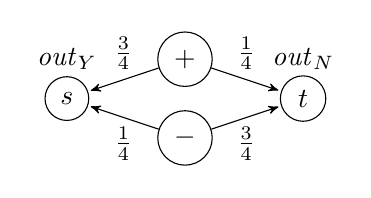
\begin{tikzpicture}[->,>=stealth',shorten >=1pt,auto,node
      distance=2cm,node/.style={circle,draw}]
      \node[node] (p) at ( 0,  .5) { $+$ };
      \node[node] (n) at ( 0, -.5) { $-$ };
      \node[node] (Y) at (-1.5,  0) { $s$ };
      \node at (-1.5, .5) { $\mathit{out}_Y$ };
      \node[node] (N) at ( 1.5,  0) { $t$ };
      \node at ( 1.5, .5) { $\mathit{out}_N$ };

      \path
      (p) edge node [above] { $\frac{3}{4}$ } (Y)
      (p) edge node [above] { $\frac{1}{4}$ } (N)
      (n) edge node [below] { $\frac{1}{4}$ } (Y)
      (n) edge node [below] { $\frac{3}{4}$ } (N)
      ;
      \end{tikzpicture}
    }
    \caption{Corresponding Markov Chain}
    \label{figure:2-dp-mdp}
  \end{subfigure}
  \caption{Survey Mechanism with $\ln 3$-Differential Privacy}
  \label{figure:2-dp}
\end{figure}

\begin{example}\label{exa:survey}
  Figure~\ref{figure:2-dp} shows the survey
mechanism and its corresponding Markov chain.
In the figure, the states
$+$ and $-$ denote the diagnoses are positive or negative
respectively; the states $s$ and $t$ denote answers to the survey
question and hence let $\mathit{out}_Y \in L (s)$ and $\mathit{out}_N
\in L (t)$.
States $+$ and $-$ are neighbors.
The random noise boosts the probability of answering
\textit{Yes} or \textit{No} to at least $1/4$ regardless of
diagnoses. Inferences on individual diagnosis can be plausibly denied.
Missing transitions (such as those from $s$ and $t$) lead
to a special state $\dagger$ with a self-loop. We omit the transitions
and the state $\dagger$ for clarity.
\end{example}


\subsection{Truncated $\alpha$-Geometric Mechanism}\label{subsec:geometric}
More sophisticated differentially private mechanisms are
available. Consider a query
$f : \mathcal{X}^n \rightarrow \bbfZ^{\geq 0}$. Let $\alpha \in (0, 1)$.
The \emph{$\alpha$-geometric mechanism}
outputs $f(x) + Y$ where $Y$ is a random variable with the geometric
distribution~\cite{GRS:09:UUPM,GRS:12:UUPM} :
\[
\Pr[Y = y] = \frac{1 - \alpha}{1 + \alpha}\alpha^{|y|}
\textmd{ for } y \in \bbfZ.
\]
The $\alpha$-geometric mechanism is oblivious since it has the same
output distribution on any inputs $x, x'$ with $f (x) = f
(x')$. Moreover, it is $(- {\Delta (f)} \ln \alpha, 0)$-differentially
private for any query $f$ with sensitivity $\Delta (f)$. The range of
the mechanism
however is $\bbfZ$. It may give nonsensical outputs such as
negative integers for queries with positive ranges.

The \emph{truncated $\alpha$-geometric mechanism over $\{ 0, 1,
  \ldots, n \}$}
outputs $f (x) + Z$ where $Z$ is a random variable with the following
distribution:
\[
\Pr[Z = z] =
\left\{
  \begin{array}{ll}
    0 & \textmd{ if } z < - f (x) \\
    \frac{\alpha^{f (x)}}{1 + \alpha} & \textmd{ if } z = -f (x)\\
    \frac{1 - \alpha}{1 + \alpha}\alpha^{|z|} &
    \textmd{ if } -f (x) < z < n - f (x)\\
    \frac{\alpha^{n - f (x)}}{1 + \alpha} & \textmd{ if } z = n-f (x)\\
    0 & \textmd{ if } z > n - f (x)
  \end{array}
\right.
\]
Note the range of the truncated $\alpha$-geometric mechanism is
$\{ 0, 1, \ldots, n \}$. The truncated $\alpha$-geometric mechanism is
again oblivious; it is also $(- {\Delta (f)} \ln \alpha, 0)$-differentially
private for any query $f$ with sensitivity $\Delta (f)$.
The truncated $\frac{1}{2}$-geometric mechanism over $\{ 0, 1, \ldots, 5 \}$ is
given in Figure~\ref{figure:geometric-mechanism-table}.

\begin{figure}[tbh]
  \centering
  \begin{subfigure}{.40\columnwidth}
    \[
    \begin{array}{|c|c|c|c|c|c|c|}
      \hline
      \textmd{input/output} & 0 & 1 & 2 & 3 & 4 & 5\\
      \hline
      0 & {2}/{3}  & {1}/{6} & {1}/{12} & {1}/{24}  & {1}/{48} & {1}/{48}\\
      \hline
      1 & {1}/{3}  & {1}/{3} & {1}/{6} & {1}/{12}  & {1}/{24} & {1}/{24}\\
      \hline
      2 & {1}/{6}  & {1}/{6} & {1}/{3} & {1}/{6}   & {1}/{12} & {1}/{12}\\
      \hline
      3 & {1}/{12} & {1}/{12} & {1}/{6} & {1}/{3}   & {1}/{6} & {1}/{6}\\
      \hline
      4 & {1}/{24} & {1}/{24} & {1}/{12} & {1}/{6}   & {1}/{3} & {1}/{3}\\
      \hline
      5 & {1}/{48} & {1}/{48} & {1}/{24} & {1}/{12} & {1}/{6} & {2}/{3}\\
      \hline
    \end{array}
    \]
    \caption{$1/2$-Geometric Mechanism}
    \label{figure:geometric-mechanism-table}
  \end{subfigure}
  \hspace{.08\columnwidth}
  \begin{subfigure}{.50\columnwidth}
    \centering
  \resizebox{.85\columnwidth}{!}{
    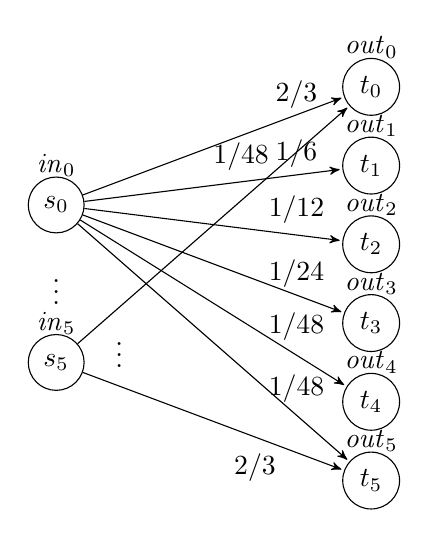
\begin{tikzpicture}[->,>=stealth',shorten >=1pt,auto,node
      distance=2cm,node/.style={circle,draw}]
      \node[node] (i0) at (0,  1) { $s_0$ };
      \node at (0, 1.5) { $\mathit{in}_0$ };
      \node at (0, 0) { $\vdots$ };
      \node at (.8, -.8) { $\vdots$ };
      \node[node] (i5) at (0, -1) { $s_5$ };
      \node at (0, -.5) { $\mathit{in}_5$ };

      \node[node] (o0) at (4,  2.5) { $t_0$ };
      \node at (4, 3) { $\mathit{out}_0$ };
      \node[node] (o1) at (4,  1.5) { $t_1$ };
      \node at (4, 2) { $\mathit{out}_1$ };
      \node[node] (o2) at (4,  0.5) { $t_2$ };
      \node at (4, 1) { $\mathit{out}_2$ };
      \node[node] (o3) at (4, -0.5) { $t_3$ };
      \node at (4, 0) { $\mathit{out}_3$ };
      \node[node] (o4) at (4, -1.5) { $t_4$ };
      \node at (4, -1) { $\mathit{out}_4$ };
      \node[node] (o5) at (4, -2.5) { $t_5$ };
      \node at (4, -2) { $\mathit{out}_5$ };

      \path
      (i0) edge node [right=30,above=10] { $2/3$ } (o0)
      (i0) edge node [right=30,above=3] { $1/6$ } (o1)
      (i0) edge node [right=30,above=-3] { $1/12$ } (o2)
      (i0) edge node [right=30,below=-5] { $1/24$ } (o3)
      (i0) edge node [right=30,below] { $1/48$ } (o4)
      (i0) edge node [right=30,below=8] { $1/48$ } (o5)

      \hide{
      (i1) edge node [above] {  } (o0)
      (i1) edge node [above] {  } (o2)
      (i1) edge node [above] {  } (o3)
      (i1) edge node [above] {  } (o4)
      (i1) edge node [above] {  } (o5)

      (i2) edge node [above] {  } (o0)
      (i2) edge node [above] {  } (o2)
      (i2) edge node [above] {  } (o3)
      (i2) edge node [above] {  } (o4)
      (i2) edge node [above] {  } (o5)

      (i3) edge node [above] {  } (o0)
      (i3) edge node [above] {  } (o2)
      (i3) edge node [above] {  } (o3)
      (i3) edge node [above] {  } (o4)
      (i3) edge node [above] {  } (o5)

      (i4) edge node [above] {  } (o0)
      (i4) edge node [above] {  } (o2)
      (i4) edge node [above] {  } (o3)
      (i4) edge node [above] {  } (o4)
      (i4) edge node [above] {  } (o5)
      }

      (i5) edge node [right=10,above=16] { $1/48$ } (o0)
      \hide{
      (i5) edge node [above] {  } (o2)
      (i5) edge node [above] {  } (o3)
      (i5) edge node [above] {  } (o4)
      }
      (i5) edge node [right=15,below=8] { $2/3$ } (o5)
      ;
      \end{tikzpicture}
    }
    \caption{Markov Chain}
    \label{figure:geometric-mechanism-markov-chain}
  \end{subfigure}
  \caption{A Markov Chain for $\frac{1}{2}$-Geometric Mechanism}
  \label{figure:geometric-mechanism}\vspace*{-.5cm}
\end{figure}

Similar to the survey mechanism, it is
straightforward to model the truncated $\frac{1}{2}$-geometric
mechanisms as Markov chains.

\begin{example}
Let the state $s_k$ and $t_l$
denote the input value $k$ and output value $l$ respectively. Define
the state set $S = \{ s_k, t_k : k \in \{ 0, 1, \ldots, n \} \}$.
The probability transition $\wp (s_k, t_l)$ is the probability of the
output value $l$ on the input value $k$ as defined in the
mechanism. Moreover, we have $\mathit{in}_k \in L (s_k)$ and
$\mathit{out}_k \in L (t_k)$ for $k \in \{ 0, 1, \ldots, n \}$.
If $\Delta (f) = 1$, $s_k$ and $s_l$ are
neighbors iff $| k - l | \leq 1$.
Figure~\ref{figure:geometric-mechanism-markov-chain} gives
the Markov chain of the truncated
$\frac{1}{2}$-geometric mechanism over $\{ 0, 1, \ldots, 5 \}$.
\end{example}

\begin{algorithm}[tbh]
	\begin{algorithmic}[1]
		\Procedure{AboveThreshold}{$d$, $t$}
		\Match{the input threshold $t$}
		\Comment{Assignments of $t'$ by $\frac{1}{4}$-geometric mechanism}
		\lCase{$0$}{$t' \leftarrow 0, 1,2,3,4,5$ with probability
			$\frac{4}{5}$,$\frac{3}{20}$,
			$\frac{3}{80}$,$\frac{3}{320}$,
			$\frac{3}{1280}$,$\frac{1}{1280}$ respectively}
		\lCase{$1$}{$t' \leftarrow 0, 1,2,3,4,5$ with probability
			$\frac{1}{5}$,$\frac{3}{5}$,
			$\frac{3}{20}$,$\frac{3}{80}$,
			$\frac{3}{320}$,$\frac{1}{320}$ respectively}
		\lCase{$2$}{$t' \leftarrow 0, 1,2,3,4,5$ with probability
			$\frac{1}{20}$,$\frac{3}{20}$,
			$\frac{3}{5}$,$\frac{3}{20}$,
			$\frac{3}{80}$,$\frac{1}{80}$ respectively}
		\lCase{$3$}{$t' \leftarrow 0, 1,2,3,4,5$ with probability
			$\frac{1}{80}$,$\frac{3}{80}$,
			$\frac{3}{20}$,$\frac{3}{5}$,
			$\frac{3}{20}$,$\frac{1}{20}$ respectively}
		\lCase{$4$}{$t' \leftarrow 0, 1,2,3,4,5$ with probability
			$\frac{1}{320}$,$\frac{3}{320}$,
			$\frac{3}{80}$,$\frac{3}{20}$,
			$\frac{3}{5}$,$\frac{1}{5}$ respectively}
		\lCase{$5$}{$t' \leftarrow 0, 1,2,3,4,5$ with probability
			$\frac{1}{1280}$,$\frac{3}{1280}$,
			$\frac{3}{320}$,$\frac{3}{80}$,
			$\frac{3}{20}$,$\frac{4}{5}$ respectively}
		\EndMatch
		\For{each query $f_i$}
		\Match{the input databese $d$}
		\Comment{Assignments of $f_{i}'$ by $\frac{1}{2}$-geometric mechanism}
		\lCase{$0$}{$f_{i}' \leftarrow 0, 1,2,3,4,5$ with probability
			$\frac{2}{3}$,$\frac{1}{6}$,
			$\frac{1}{12}$,$\frac{1}{24}$,
			$\frac{1}{48}$,$\frac{1}{48}$ respectively}
		\lCase{$1$}{$f_{i}' \leftarrow 0, 1,2,3,4,5$ with probability
			$\frac{1}{3}$,$\frac{1}{3}$,
			$\frac{1}{6}$,$\frac{1}{12}$,
			$\frac{1}{24}$,$\frac{1}{24}$ respectively}
		\lCase{$2$}{$f_{i}' \leftarrow 0, 1,2,3,4,5$ with probability
			$\frac{1}{6}$,$\frac{1}{6}$,
			$\frac{1}{3}$,$\frac{1}{6}$,
			$\frac{1}{12}$,$\frac{1}{12}$ respectively}
		\lCase{$3$}{$f_{i}' \leftarrow 0, 1,2,3,4,5$ with probability
			$\frac{1}{12}$,$\frac{1}{12}$,
			$\frac{1}{6}$,$\frac{1}{3}$,
			$\frac{1}{6}$,$\frac{1}{6}$ respectively}
		\lCase{$4$}{$f_{i}' \leftarrow 0, 1,2,3,4,5$ with probability
			$\frac{1}{24}$,$\frac{1}{24}$,
			$\frac{1}{12}$,$\frac{1}{6}$,
			$\frac{1}{3}$,$\frac{1}{3}$ respectively}
		\lCase{$5$}{$f_{i}' \leftarrow 0, 1,2,3,4,5$ with probability
			$\frac{1}{48}$,$\frac{1}{48}$,
			$\frac{1}{24}$,$\frac{1}{12}$,
			$\frac{1}{6}$,$\frac{2}{3}$ respectively}
		\EndMatch
		\If{$f_{i}'>t'$}
		\State{$a_i=\top$}
		\State{\Return}
		\Else
		\State{$a_i=\bot$}
		\EndIf
		\EndFor
		\EndProcedure
		
	\end{algorithmic}
	\caption{Input is a private database $d \in \{0,1,\ldots,5\}$, an adaptively chosen stream of sensitivity 1 queries $f_1,f_2$,\ldots, a threshold $t \in \{0,1,\ldots,5\}$. Output is a stream of answers $a_1,a_2$,\ldots}
	\label{algorithm:online-model}
\end{algorithm}

\subsection{Above Threshold Mechanism}
In the differentially privacy context, we differentiate between \emph{offline} and \emph{online} models.
In the offline (or \emph{non-interactive}) model the curator releases the outputs only once and plays no further role. Thus the models we constructed in previous section are offline models. On the contrary, in the online (or \emph{interactive}) model the curator can permit further queries. In this setting it is obvious that queries do not change database themselves. To maintain differential privacy, the curator however can decide to change data analysis mechanisms accordingly. For instance, after a certain output is disclosed or a certain number of queries, it may decide to disable further queries.

Below we describe an online model adapted from~\cite{DR:14:AFDP}: it is used in the scenario where a large amount of queries occur, but we only care for the queries which
are above a given threshold. Other queries below the threshold are considered \emph{irrelevant} and won't cause privacy disclosure. In~\cite{DR:14:AFDP}, the model is set for continuous database, and the Laplace mechanisms are applied to both queries and the threshold. In our model, the database is discrete and instead the geometric mechanisms are applied.

We consider the database set $D = \{0,1\ldots,5\}$, a threshold $t \in \{0,1\ldots,5\}$, and queries $\{f| f $ with sensitivity $\Delta (f) = 1 \}$. In order to protect privacy, truncated $\alpha$-geometric mechanisms over $\{0,1\ldots,5\}$ are applied to each query and the threshold, and what we observe is the first time that a query result is greater than or equal to the threshold after interference. We are interested in the differentially private property of the data in $D$, assuming that a pair of data $d,d'$are neighbors, if $|d-d'|\le 1$. The algorithm is shown in Algorithm~\ref{algorithm:online-model} and a property will be specefied in Section~\ref{section:specifying-properties}.







\section{The Logic $\dpCTL$}
\label{section:dpCTL}

The logic $\dpCTL$ is designed to specify differentially private
mechanisms. We introduce the differentially private path quantifer
$\dpriv{\epsilon}{\delta}$ in $\dpCTL$. For any path formula
$\phi$, a state $s$ in a Markov chain $K$ satisfies
$\dpriv{\epsilon}{\delta} \phi$ if the probability of having $\phi$-paths 
from $s$ is close to the probabilities of 
having $\phi$-paths from its neighboring states. 
We give semantics for both Markov chains and Markov decision processes. 



\subsection{Syntax}
\label{subsection:syntax}

The syntax of $\dpCTLstar$ state and path formulae is given by:
\begin{eqnarray*}
  \Phi & ::= & p \ |\ \neg \Phi \ |\ \Phi \wedge \Phi \ |\
               \PJ{J} \phi \ |\ \dpriv{\epsilon}{\delta} \phi\\
  \phi & ::= & \Phi \ |\ \neg\phi  \ |\  \phi\wedge\phi  \ |\  \X \phi \ |\ \phi \until \phi
\end{eqnarray*}
A \emph{state} formula $\Phi$ is either  an atomic proposition
$p$, the negation of a state formula, the conjunction of two state
formulae, the \emph{probabilistic} operator $\PJ{J}$ with $J$
an interval in $[0, 1]$ followed by a path formula, or the
\emph{differentially private} operator $\dpriv{\epsilon}{\delta}$
 with two non-negative real numbers $\epsilon$ and $\delta$ followed
 by a path formula. A
\emph{path} formula $\phi$ is simply a linear temporal logic formula, with temporal operator \emph{next}  ($\X$)
and  \emph{until} operator
($\until$) operator enclosed by two path formulae.
We moreover define $F \phi \equiv true \until \phi$ and $G\phi \equiv \neg F (\neg\phi)$.

As in the classical setting, we consider the sublogic $\dpCTL$ by allowing only path formulae of the form $\X\Phi$ and $\Phi\until\Phi$.
Moreover, one obtains $\PCTL$~\cite{HanssonJ94} and $\PCTLstar$~\cite{BiancoA95} from $\dpCTL$ and $\dpCTLstar$
by removing the differentially private operator  $\dpriv{\epsilon}{\delta}$.



\subsection{Semantics}
\label{subsection:semantics}

Given a finite discrete-time Markov chain $K = (S, \wp, L)$, a
\emph{neighborhood relation on $S$} $\neighbor{S} \subseteq S \times S$
is a reflexive and symmetric relation on $S$. We will write $s
\neighbor{S} t$ when $(s, t) \in \neighbor{S}$. If $s \neighbor{S} t$,
we say $s$ and $t$ are \emph{neighbors} or $t$ is a \emph{neighbor} of
$s$. Define the satisfaction relation $K, \neighbor{S}, s
\models \Phi$ as follows.
\begin{eqnarray*}
  K, \neighbor{S}, s \models \top\\
  K, \neighbor{S}, s \models p
  & \textmd{ if } &
  p \in L(s)\\
  K, \neighbor{S}, s \models \neg \Phi
  & \textmd{ if } &
  K, \neighbor{S}, s \not\models \Phi\\
  K, \neighbor{S}, s \models \Phi_0 \wedge \Phi_1
  & \textmd{ if } &
  K, \neighbor{S}, s \models \Phi_0 \textmd{ and }
  K, \neighbor{S}, s \models \Phi_1\\
  K, \neighbor{S}, s \models \PJ{J} \phi
  & \textmd{ if } &
  \Pr [\{ \pi : K, \neighbor{S}, \pi \models \phi \textmd{ with }
                    \pi_0 = s\}] \in J \\
  K, \neighbor{S}, s \models \dpriv{\epsilon}{\delta} \phi
  & \textmd{ if } &
  \textmd{for every } t \textmd{ with }  s \neighbor{S} t,
      p(s) \leq e^{\epsilon} p(t) + \delta \textmd{ and }
      p(t) \leq e^{\epsilon} p(s)  +  \\
  & &  \delta \textmd{ where } p(x) = \Pr [\{
      \pi : K, \neighbor{S}, \pi \models \phi \textmd{ with}
      \pi_0 = x \}]
\end{eqnarray*}

Moreover, the relation $K, \neighbor{S}, \pi \models \phi$ is defined as
for the standard LTL formulas~\cite{which-to-cite?}. We only recall the semantics for $\X$ and $\until$ as follows.
\begin{eqnarray*}
  K, \neighbor{S}, \pi \models \X \phi
  & \textmd{ if } &
  K, \neighbor{S}, \pi[1] \models \phi\\
  K, \neighbor{S}, \pi \models \phi \until \psi
  & \textmd{ if } &
  \textmd{there is a } j \geq 0 \textmd{ such that }
  K, \neighbor{S}, \pi[j] \models \psi \textmd{ and } \\
  & & K, \neighbor{S}, \pi[k] \models \phi
      \textmd{ for every } 0 \leq k < j
\hide{
  K, \neighbor{S}, \pi \models \Phi \buntil{n} \Psi
  & \textmd{ if } &
  \textmd{there is a } 0 \leq j \leq n \textmd{ such that }
  K, \neighbor{S}, \pi[j] \models \Psi \textmd{ and } \\
  & & K, \neighbor{S}, \pi[k] \models \Phi
      \textmd{ for every } 0 \leq k < j
}
\end{eqnarray*}

To simplify our notation, for any Markov chain $K$, neighborhood
relation $N$ on $S$, a state $s \in S$, and a path formula $\phi$,
define
\[
\myPr{s}{K}{N}{\phi} =
\Pr [ \{ \pi : K, N, \pi \models \phi \textmd{ with } \pi_0 = s \} ].
\]
That is, $\myPr{s}{K}{N}{\phi}$ denotes the probability of paths
satisfying $\phi$ from $s$ on $K$ with $N$. The semantics of the
differentially private operator hence becomes
\begin{eqnarray*}
  K, \neighbor{S}, s \models \dpriv{\epsilon}{\delta} \phi
  & \textmd{ if } &
  \textmd{for every } t \textmd{ with }  s \neighbor{S} t,
      \myPr{s}{K}{N}{\phi} \leq e^{\epsilon} \myPr{t}{K}{N}{\phi} + \delta
      \textmd{ and }\\
  & &  \myPr{t}{K}{N}{\phi} \leq e^{\epsilon} \myPr{s}{K}{N}{\phi} + \delta
\end{eqnarray*}

Other than the differentially private operator, the semantics of
$\dpCTLstar$ is standard~\cite{BK:08:PMC}.
To intuit the semantics of $\dpriv{\epsilon}{\delta} \phi$,
recall that  $\myPr{s}{K}{N}{\phi}$ is the probability of having
paths satisfying $\phi$ from $s$. Thus, a state $s$ satisfies
$\dpriv{\epsilon}{\delta} \phi$ if having paths satisfying $\phi$
from $s$ is $(\epsilon, \delta)$-close to having paths satisfying
$\phi$ from every neighbor of $s$. In other words, it is
probabilistically similar to observe paths satisfying $\phi$ from $s$
and from all neighbors of $s$.

\subsection{Model Checking Algorithms}
We first describe the model checking algorithm for $\dpCTL$, which follows the classical
algorithms for $\PCTL$ by computing the states satisfying
sub state-formulae inductively~\cite{BK:08:PMC}. It hence suffices to
consider the inductive step where the states satisfying the subformula
$\dpriv{\epsilon}{\delta} (\phi)$ is computed.

%We start with the algorithm for Markov chains.

In the classical $\PCTL$ model checking algorithm for Markov chains,
states satisfying the subformula $\PJ{J} \phi$ are obtained by
computing $\myPr{s}{K}{\neighbor{S}}{\phi}$ for state $s \in S$.
These probabilities can be computed by solving linear equations or
through iterative approximations. We summarize it in the following
theorem~\cite{BK:08:PMC}:

\begin{lemma}
  Let $K = (S, \wp, L)$ be a Markov chain, $s
  \in S$, and $B, C \subseteq S$. The probabilities
  $\myPr{s}{K}{\neighbor{S}}{\gX B}$ and
  $\myPr{s}{K}{\neighbor{S}}{B \mho C}$
\hide{
  $\Pr[\{ \pi : K, \neighbor{K}, \pi \models B \buntil{n} C \textmd{
    with } \pi_0 = s \}]$
} are computable within time polynomial in
  $|S|$.
  \label{lemma:PJ-subroutines}
\end{lemma}

In Lemma~\ref{lemma:PJ-subroutines}, we abuse the notation slightly to
admit path formulae of the form $\gX B$ (next $B$) and
$B \guntil C$ ($B$ until $C$) with $B, C \subseteq S$ as
in~\cite{BK:08:PMC}. They are interpreted by introducing new atomic
propositions $B$ and $C$ for each $s \in B$ and $s \in C$
respectively. 
\hide{
We will also use graphical symbols $\gF C$ ($C$ in
the future) and $\gG C$ (globally $C$) in such path formulae
$\varphi$ to minimize confusion.
}

In order to determine the set $\{ s : K, \neighbor{S}, s \models
\dpriv{\epsilon}{\delta} \varphi \}$, our algorithm first computes
the probabilities $p (s) = \myPr{s}{K}{\neighbor{S}}{\varphi}$ for every
$s \in S$ (Algorithm~\ref{algorithm:sat-dpriv-dtmc}). For each $s \in S$,
it then compares the probabilities $p (s)$ and $p (t)$ for every
neighbor $t$ of $s$. If there is a neighbor $t$ such that $p (s)$ and
$p (t)$ are not $(\epsilon, \delta)$-close, the state $s$
is removed from the result. Hence
Algorithm~\ref{algorithm:sat-dpriv-dtmc} returns all states which are
$(\epsilon, \delta)$-close to their neighbors.
The algorithm requires at most $O
(|S|^2)$ additional steps. We hence have the following results:

\begin{algorithm}
  \begin{algorithmic}[1]
    \Function{SAT}{$K$, $\neighbor{S}$, $\phi$}
    \Match{$\phi$}
    \Comment{by Lemma~\ref{lemma:PJ-subroutines}}
    \Case{$\X \Psi$}
      \State{$B \leftarrow \textmd{SAT} (K, \neighbor{S}, \Psi)$}
      \State{$p(s) \leftarrow \myPr{s}{K}{\neighbor{S}}{\gX B}$
        for every $s \in S$}
    \EndCase
    \Case{$\Psi \until \Psi'$}
      \State{$B \leftarrow \textmd{SAT} (K, \neighbor{S}, \Psi)$}
      \State{$C \leftarrow \textmd{SAT} (K, \neighbor{S}, \Psi')$}
      \State{$p(s) \leftarrow \myPr{s}{K}{\neighbor{S}}{B \guntil C}$ for
        every $s \in S$}
    \EndCase
    \EndMatch
    \State{$R \leftarrow S$}
    \For{$s \in S$}
      \For{$t$ with $s \neighbor{K} t$}
        \If{$p(s) \not\leq e^{\epsilon} p(t) + \delta$ or
            $p(t) \not\leq e^{\epsilon} p(s) + \delta$}
        {remove $s$ from $R$}
        \EndIf
      \EndFor
    \EndFor

    \State{\Return $R$}
    \EndFunction
  \end{algorithmic}
  \caption{SAT($\phi$, $\neighbor{K}$)}
  \label{algorithm:sat-dpriv-dtmc}
\end{algorithm}

\begin{proposition}
  Let $K = (S, \wp, L)$ be a Markov chain.
  $\{ s : K, \neighbor{K}, s \models \dpriv{\epsilon}{\delta} \phi \}$ is
  computable within time polynomial in $|S|$.
\end{proposition}

\begin{corollary}
  Let $K = (S, \wp, L)$ be a Markov chain and $\Phi$ a $\dpCTL$
  formula. $\{ s : K, \neighbor{K}, s \models \Phi \}$ is
  computable within time polynomial in $|S|$ and $|\Phi|$.
\end{corollary}

The model checking algorithm for $\dpCTLstar$ can be treated as in the classical setting~\cite{BK:08:PMC}:  all we need is to  compute the  probability
  $\myPr{s}{K}{\neighbor{S}}{\phi}$ with general path formula $\phi$. For this purpose one first constructs a deterministic $\omega$-automaton $R$, such as deterministic Rabin automaton. Then, the probability reduces to a
  reachability probability in the product Markov chain obtained from $K$ and $R$. There are more efficient algorithms without the product construction, see \cite{CY95,CSS03,BaierKKKMW16} for details.


\section{Model Checking Algorithms}
\label{section:model-checking-algorithms}

The model checking algorithms for $\dpCTL$ follow the classical
algorithms for $\PCTL$ by computing the states satisfying 
sub state-formulae inductively~\cite{BK:08:PMC}. It hence suffices to
consider the inductive step where the states satisfying the subformula 
$\dpriv{\epsilon}{\delta} (\phi)$ is computed. We start with the
algorithm for Markov chains.

In the classical $\PCTL$ model checking algorithm for Markov chains,
states satisfying the subformula $\PJ{J} \phi$ are obtained by
computing $\myPr{s}{K}{\neighbor{S}}{\phi}$ for state $s \in S$. 
These probabilities can be computed by solving linear equations or
through iterative approximations. We summarize it in the following
theorem~\cite{BK:08:PMC}:

\begin{lemma}
  Let $K = (S, \wp, L)$ be a Markov chain, $s
  \in S$, and $B, C \subseteq S$. The probabilities
  $\myPr{s}{K}{\neighbor{S}}{\gX B}$ and
  $\myPr{s}{K}{\neighbor{S}}{B \mho C}$
\hide{
  $\Pr[\{ \pi : K, \neighbor{K}, \pi \models B \buntil{n} C \textmd{
    with } \pi_0 = s \}]$ 
} are computable within time polynomial in
  $|S|$.
  \label{lemma:PJ-subroutines}
\end{lemma}

In Lemma~\ref{lemma:PJ-subroutines}, we abuse the notation slightly to
admit path formulae of the form $\gX B$ (next $B$) and
$B \guntil C$ ($B$ until $C$) with $B, C \subseteq S$ as
in~\cite{BK:08:PMC}. They are interpreted by introducing new atomic
propositions $B$ and $C$ for each $s \in B$ and $s \in C$
respectively. We will also use graphical symbols $\gF C$ ($C$ in
the future) and $\gG C$ (globally $C$) in such path formulae
$\varphi$ to minimize confusion.  

In order to determine the set $\{ s : K, \neighbor{S}, s \models
\dpriv{\epsilon}{\delta} \varphi \}$, our algorithm first computes
the probabilities $p (s) = \myPr{s}{K}{\neighbor{S}}{\varphi}$ for every
$s \in S$ (Algorithm~\ref{algorithm:sat-dpriv-dtmc}). For each $s \in S$,
it then compares the probabilities $p (s)$ and $p (t)$ for every
neighbor $t$ of $s$. If there is a neighbor $t$ such that $p (s)$ and
$p (t)$ are not $(\epsilon, \delta)$-close, the state $s$
is removed from the result. Hence
Algorithm~\ref{algorithm:sat-dpriv-dtmc} returns all states which are
$(\epsilon, \delta)$-close to their neighbors. 
The algorithm requires at most $O
(|S|^2)$ additional steps. We hence have the following results:

\begin{algorithm}
  \begin{algorithmic}[1]
    \Function{SAT}{$K$, $\neighbor{S}$, $\phi$}
    \Match{$\phi$}
    \Comment{by Lemma~\ref{lemma:PJ-subroutines}}
    \Case{$\X \Psi$} 
      \State{$B \leftarrow \textmd{SAT} (K, \neighbor{S}, \Psi)$}
      \State{$p(s) \leftarrow \myPr{s}{K}{\neighbor{S}}{\gX B}$
        for every $s \in S$} 
    \EndCase
    \Case{$\Psi \until \Psi'$}
      \State{$B \leftarrow \textmd{SAT} (K, \neighbor{S}, \Psi)$}
      \State{$C \leftarrow \textmd{SAT} (K, \neighbor{S}, \Psi')$}
      \State{$p(s) \leftarrow \myPr{s}{K}{\neighbor{S}}{B \guntil C}$ for
        every $s \in S$} 
    \EndCase
    \EndMatch
    \State{$R \leftarrow S$}
    \For{$s \in S$}
      \For{$t$ with $s \neighbor{K} t$}
        \If{$p(s) \not\leq \epsilon p(t) + \delta$ or
            $p(t) \not\leq \epsilon p(s) + \delta$}
        {remove $s$ from $R$}
        \EndIf
      \EndFor
    \EndFor
    
    \State{\Return $R$}
    \EndFunction
  \end{algorithmic}
  \caption{SAT($\phi$, $\neighbor{K}$)}
  \label{algorithm:sat-dpriv-dtmc}
\end{algorithm}

\begin{proposition}
  Let $K = (S, \wp, L)$ be a Markov chain.
  $\{ s : K, \neighbor{K}, s \models \dpriv{\epsilon}{\delta} \phi \}$ is
  computable within time polynomial in $|S|$.
\end{proposition}

\begin{corollary}
  Let $K = (S, \wp, L)$ be a Markov chain and $\Phi$ a $\dpCTL$
  formula. $\{ s : K, \neighbor{K}, s \models \Phi \}$ is
  computable within time polynomial in $|S|$ and $|\Phi|$.
\end{corollary}

Our next task is to compute $\{ M, \neighbor{S}, s \models
\dpriv{\epsilon}{\delta} \phi \}$ for a Markov decision process $M =
(S, \Act, \wp, L)$. Recall the semantics of $\dpriv{\epsilon}{\delta}
\phi$. Given $s, t$ with $s \neighbor{M} t$ and a path formula
$\phi$, we need to decide whether
$\myPr{s}{M_{\scheduler{S}}}{\neighbor{S}}{\phi} \leq 
\epsilon \myPr{t}{M_{\scheduler{S}}}{\neighbor{S}}{\phi} + \delta$
for every scheduler $\scheduler{S}$. 
By recursion, we will obtain a
(generalized) path formula $\varphi$ from $\phi$. It suffices to
decide whether 
$\myPr{s}{M_{\scheduler{S}}}{\neighbor{S}}{\varphi} \leq 
\epsilon \myPr{t}{M_{\scheduler{S}}}{\neighbor{S}}{\varphi} + \delta$.
To do so, we will find a position-independent strategy $\scheduler{S}$
maximizing $\myPr{s}{M_{\scheduler{S}}}{\neighbor{S}}{\varphi} -
\epsilon \myPr{t}{M_{\scheduler{S}}}{\neighbor{S}}{\varphi}$ and check
if the maximum is less than or equal to $\delta$. 
As a starter, consider
\begin{eqnarray}
  \label{eqn:max-nextB}
\max_{\textmd{pos.-ind. } \scheduler{S}} 
\myPr{s}{M_{\scheduler{S}}}{\neighbor{S}}{\gX B} -
\epsilon \myPr{t}{M_{\scheduler{S}}}{\neighbor{S}}{\gX B}
\end{eqnarray}
where $s, t \in S$ and $B \subseteq S$. To compute
(\ref{eqn:max-nextB}), one has to consider paths satisfying $\gX B$ 
from $s$ and $t$ induced by the same action sequences. In the
following, we construct the self-product of Markov decision
processes. Similar to product automata, the product MDP simulates
probabilistic computation from $s$ and $t$ on the same actions in
parallel. A strategy on the product MDP corresponds to a
position-independent strategy in the original MDP. 

Let $M = (S, \Act, \wp, L)$ be a reactive MDP.
Define the \emph{self-product} MDP
$M^{\times} = (S \times S, \Act, \wp^{\times}, \emptyset)$ where
$\wp^{\times} ((s, t), \alpha, (s', t')) = \wp (s, \alpha, s') \times
\wp (t, \alpha, 
t')$. Observe that $\sum_{(s', t') \in S \times S} \wp^{\times} ((s, t),
\alpha, (s', t'))$ $=$ $\sum_{s' \in S} \sum_{t' \in S} \wp (s, \alpha,
s') \times \wp (t, \alpha, t')$ $=$ $\sum_{s' \in S}$ $\wp (s, \alpha, s')
\sum_{t' \in S} \wp (t, \alpha, t')$ $=$ $\sum_{s' \in S} \wp (s, \alpha,
s')$ $=$ $1$. $\wp^{\times} ((s, t), \alpha, \bullet)$ is a probability
distribution over $S \times S$ for every $\alpha \in \Act$.

\begin{lemma}
  Let $M = (S, \Act, \wp, L)$ be a reactive Markov decision process and
  $M^{\times}$ its self-product. For any paths $s_0\alpha_1s_1\alpha_2
  \cdots \alpha_k s_k$ and $t_0 \alpha_1 t_1 \alpha_2 \cdots \alpha_k
  t_k$ induced by $\alpha_1 \alpha_2 \cdots \alpha_k$, we have
  $\Pr^{M} [s_0 \alpha_1 s_1 \alpha_2 \cdots \alpha_k s_k] \times
  \Pr^{M} [t_0 \alpha_1 t_1 \alpha_2 \cdots \alpha_k t_k] =
  \Pr^{M^{\times}} [(s_0, t_0) \alpha_1 (s_1, t_1) \alpha_2 \cdots
  \alpha_k (s_k, t_k)]$.
  \label{lemma:joint-probability}
\end{lemma}

\todo{Correspondence between strategies on $M$ and $M^{\times}$}

Since strategies on $M^{\times}$ are position-independent strategies
on $M$, we compute (\ref{eqn:max-nextB}) by finding the maximal
expected reward on $M^{\times}$ of infinite time horizon with absoring
states. A \emph{reward function} on $M$ is a function $r : S
\rightarrow \bbfR$. For an $\scheduler{S}$-path $\pi = \pi_0 \alpha_1 \pi_1
\cdots$, define $r (\pi) = \sum_i r (\pi_i)$.
Let $\mathit{Ab} \subseteq S$. Define $M[\mathit{Ab}] = (S, \Act,
\wp^-, L)$ where $\wp^- (s, \alpha, t) = \wp (s, \alpha, t)$ if $s
\not\in \mathit{Ab}$ and $\wp^- (s, \alpha, t) = 0$ otherwise. That
is, $M[\mathit{Ab}]$ is an MDP with the \emph{absorbing} states
$\mathit{Ab}$. 
For any scheduler $\scheduler{S}$, the expected reward on $M$ of
infinite time horizon with absorbing states is
\begin{eqnarray*}
{V}^{\scheduler{S}} (s) & = & 
E[ {r} (\pi) | \pi
\textmd{ is an $\scheduler{S}$-path of } M[\mathit{Ab}]
\textmd{ with } \pi_0 = s ]
\end{eqnarray*}

Consider the following reward functions on $M^{\times}$:
\[
\begin{array}{c|ccccc}
  \textmd{when } (s, t) \in 
  & B \times (S \setminus B)
  & \hspace{1em}
  & (S \setminus B) \times B
  & \hspace{1em}
  & \textmd{others}\\
  \hline
  {r}_{\gX B, S}^{\times} (s, t) & 1 && 0 && 0\\
  {r}_{S, \gX B}^{\times} (s, t) & 0 && -\epsilon && 0\\
\end{array}
\]
Let $\nevernextB = \{ s : M, s \models \forall \gX (S \setminus
B) \}$, $\mathit{Ab}_{\gX B, \gX B} = (B
\times B) \cup (B \times \nevernextB) \cup (\nevernextB \times B)
\cup (\nevernextB \times \nevernextB)$.
Define
\begin{eqnarray*}
  {V}_{\gX B, S}^{\times \scheduler{S}} (s, t) & = &
  E[ {r}_{\gX B, S}^{\times} (\pi^{\times}) | \pi^{\times} \textmd{ is an
  $\scheduler{S}$-path of } M^{\times}[\mathit{Ab}_{\gX B, \gX B}]
  \textmd{ with } \pi_0^{\times} = (s, t) ]\\
  {V}_{S, \gX B}^{\times \scheduler{S}} (s, t) & = &
  E[ {r}_{S, \gX B}^{\times} (\pi^{\times}) | \pi^{\times} \textmd{ is an
  $\scheduler{S}$-path of } M^{\times}[\mathit{Ab}_{\gX B, \gX B}] 
  \textmd{ with } \pi_0^{\times} = (s, t) ]
\end{eqnarray*}

The expected rewards ${V}_{\gX, S}^{\times\scheduler{S}} (s, t)$ and
${V}_{S, \gX}^{\times\scheduler{S}} (s, t)$ are the weighted
probabilities of having $\gX B$-paths from $s$ and $t$
respectively. More formally,
\begin{proposition}
  \label{proposition:joint-probabilities}
  Let $M = (S, \Act, \wp, L)$ be a reactive MDP and $B \subseteq S$.
  For any scheduler $\scheduler{S}$ on $M^{\times}$, we have
  \begin{enumerate}
  \item ${V}_{\gX B, S}^{\times\scheduler{S}} (s, t) = 
    \myPr{s}{M_{\scheduler{S}}}{\neighbor{S}}{\gX B}$;
  \item ${V}_{S, \gX B}^{\times\scheduler{S}} (s, t) =  
    -\epsilon \cdot \myPr{t}{M_{\scheduler{S}}}{\neighbor{S}}{\gX B}$.
  \end{enumerate}
\end{proposition}

, and $S^{?}_{\gX B} = S
\times S \setminus \mathit{Ab}_{\gX B}$
\begin{eqnarray}
  \label{eqn:lp-nextB}
\begin{array}{rclll}
  \multicolumn{3}{c}{
  \min \sum\limits_{(s, t) \in {S}^{?}_{\gX B}} x_{s, t}
  }\\
  x_{s, t} & = & 0 & \hspace{.05\columnwidth} &
  (s, t) \in \nevernextB \times \nevernextB \\
  x_{s, t} & = & 1 && 
  (s, t) \in B \times \nevernextB\\
  x_{s, t} & = & - \epsilon &&
  (s, t) \in \nevernextB \times B\\
  x_{s, t} & = & 1 - \epsilon && 
  (s, t) \in B \times B\\
  x_{s, t} &\geq& 
  \sum\limits_{(s', t') \in {S}^{2}}
   \wp^{\times} ((s, t), \alpha, (s', t')) \times x_{s', t'} 
  &&
  \alpha \in \Act, (s, t) \in {S}^{?}_{\gX B}
\end{array}
\end{eqnarray}

\begin{theorem}
  Let $x^*_{s, t}$ attain the optimum in the linear programming
  problem~(\ref{eqn:lp-nextB}). For every $s, t \in S$, 
  $x^*_{s, t} = \max\limits_{\scheduler{S}}
  \myPr{s}{M_{\scheduler{S}}}{\neighbor{S}}{\gX B} - 
  \epsilon \myPr{t}{M_{\scheduler{S}}}{\neighbor{S}}{\gX B}$.  
  \label{theorem:nextC}
\end{theorem}

Next, we consider the generalized path formula $\varphi = \gF C$. We
would like to compute the maximal difference of weighted probabilities
of paths satisfying $\gF C$ from $s$ and $t$ among
position-independent schedulers. That is, 
\begin{eqnarray}
  \label{eqn:max-eventuallyC}
\max_{\textmd{pos.-ind. } \scheduler{S}} 
\myPr{s}{M_{\scheduler{S}}}{\neighbor{S}}{\gF C} -
\epsilon \myPr{t}{M_{\scheduler{S}}}{\neighbor{S}}{\gF C}
\end{eqnarray}
where $s, t \in S$ and $C \subseteq S$. 

Let $M = (S, \Act, \wp, L)$ and $C \subseteq S$. Define $\lift{M}{C} =
((S \setminus C) \cup \{ \bot, \top \}, \Act, \lift{\wp}{C}, \lift{L}{C})$ where
$\lift{L}{C} (s) = L (s)$ for $s \in S$ and $\lift{L}{C} (\bot) =
\lift{L}{C} (\top) = \emptyset$; and
\begin{itemize}
\item $\lift{\wp}{C} (s, \alpha, t) = \wp (s, \alpha, t)$ for $s \in
  S$, $\alpha \in \Act$ and $t \not\in C$;
\item $\lift{\wp}{C} (s, \alpha, \top) = \sum_{t \in C} \wp (s,
  \alpha, t)$ for $s \in S$, $\alpha \in \Act$; and
\item $\lift{\wp}{C} (\top, \alpha, \bot) = \lift{\wp}{C} (\bot,
  \alpha, \bot) = 1$ for $\alpha \in \Act$.
\end{itemize}

Consider the following reward functions on $\lift{M}{C}^{\times}$:
\[
\begin{array}{c|cccccccc}
  \textmd{when } (s, t) \in 
  & \{ \top \} \times (S \setminus C)
  & \hspace{1em}
  & (S \setminus C) \times \{ \top \}
  & \hspace{1em}
  & \{ (\top, \top) \}
  & \hspace{1em}
  & \textmd{others}\\
  \hline
  {r}_{{\gF C}S}^{\times} (s, t) & 1 && 0 && 1 && 0\\
  {r}_{S{\gF C}}^{\times} (s, t) & 0 && -\epsilon && -\epsilon && 0\\
  {r}_{{\gF C}{\gF C}}^{\times} (s, t) & 1 && -\epsilon && 1-\epsilon && 0\\
\end{array}
\]
Let $\mathit{Ab}_{\gF C, \gF C} = \{ \bot, \top \} \times \{ \bot,
\top \} \cup \{ \bot, \top \} \times \neverC \cup \neverC \times \{
\bot, \top \} \cup \neverC \times \neverC$ be the absorbing states.
Define
\begin{eqnarray*}
  {V}_{\gF C, S}^{\times \scheduler{S}} (s, t) & = &
  E[ {r}_{\gF C, S}^{\times} (\pi^{\times}) | \pi^{\times} \textmd{ is an
  $\scheduler{S}$-path of } M^{\times}[\mathit{Ab}_{\gF C, \gF C}]
  \textmd{ with } \pi_0^{\times} = (s, t) ]\\
  {V}_{S, \gF C}^{\times \scheduler{S}} (s, t) & = &
  E[ {r}_{S, \gF C}^{\times} (\pi^{\times}) | \pi^{\times} \textmd{ is an
  $\scheduler{S}$-path of } M^{\times}[\mathit{Ab}_{\gF C, \gF C}] 
  \textmd{ with } \pi_0^{\times} = (s, t) ]\\
  {V}_{\gF C, \gF C}^{\times \scheduler{S}} (s, t) & = &
  E[ {r}_{\gF C, \gF C}^{\times} (\pi^{\times}) | \pi^{\times} \textmd{ is an
  $\scheduler{S}$-path of } M^{\times}[\mathit{Ab}_{\gF C, \gF C}] 
  \textmd{ with } \pi_0^{\times} = (s, t) ]
\end{eqnarray*}

\begin{proposition}
  Let $M = (S, \Act, \wp, L)$ be a reactive MDP and $C \subseteq S$.
  For any scheduler $\scheduler{S}$ on $M^{\times}$, we have
  \begin{enumerate}
  \item ${V}_{\gF C, S}^{\times\scheduler{S}} (s, t) = 
    \myPr{s}{M_{\scheduler{S}}}{\neighbor{S}}{\gF C}$;
  \item ${V}_{S, \gF C}^{\times\scheduler{S}} (s, t) =  
    -\epsilon \cdot \myPr{t}{M_{\scheduler{S}}}{\neighbor{S}}{\gF C}$.
  \end{enumerate}
  \label{proposition:individual-probability-nextC}
\end{proposition}

Observe that ${r}_{\gF C, \gF C}^{\times \scheduler{S}} (s, t) =
{r}_{\gF C, S}^{\times \scheduler{S}} (s, t) + {r}_{S, \gF C}^{\times
  \scheduler{S}} (s, t)$. By linearity of expectation, we have
\begin{eqnarray*}
  & & {V}_{\gF C, \gF C}^{\times \scheduler{S}} (s, t)\\
  &=& E[ {r}_{\gF C, \gF C}^{\times \scheduler{S}} (\pi^{\times}) |
      \pi^{\times} \textmd{ is an $\scheduler{S}$-path of }
      M^{\times}[\mathit{Ab}_{\gF C, \gF C}] \textmd{ with }
      \pi_0^{\times} = (s, t) ]\\
  &=&  E[ {r}_{\gF C, S}^{\times \scheduler{S}} (\pi^{\times}) |
      \pi^{\times} \textmd{ is an $\scheduler{S}$-path of }
      M^{\times}[\mathit{Ab}_{\gF C, \gF C}] \textmd{ with }
      \pi_0^{\times} = (s, t) ] +\\
  & &  E[ {r}_{S, \gF C}^{\times \scheduler{S}} (\pi^{\times}) |
      \pi^{\times} \textmd{ is an $\scheduler{S}$-path of }
      M^{\times}[\mathit{Ab}_{\gF C, \gF C}] \textmd{ with }
      \pi_0^{\times} = (s, t) ]\\
  &=& {V}_{\gF C, S}^{\times \scheduler{S}} (s, t) +
      {V}_{S, \gF C}^{\times \scheduler{S}} (s, t)\\
  &=& \myPr{s}{M_{\scheduler{S}}}{\neighbor{S}}{\gF C} -
      \epsilon \cdot \myPr{t}{M_{\scheduler{S}}}{\neighbor{S}}{\gF C}.
\end{eqnarray*}


\begin{lemma}
  Let $M = (S, \Act, \wp, L)$ be a reactive MDP and $C \subseteq S$.
  For any scheduler $\scheduler{S}$ on $M$,
  $V^{\scheduler{S}}_{\Diamond C} (s, t) =
  \myPr{s}{M_{\scheduler{S}}}{\neighbor{S}}{\gF C} -
  \epsilon \myPr{t}{M_{\scheduler{S}}}{\neighbor{S}}{\gF C}$.
\label{lemma:eventuallyC}
\end{lemma}

With Lemma~\ref{lemma:eventuallyC}, it is standard to compute 
the maximal value (\ref{eqn:max-eventuallyC}) by linear programming.
Let ${S}^{?}_{\Diamond C} = S \times S \setminus
\mathit{Ab}_{\Diamond C}$. Consider the following 
instance of the linear programming problem:
\begin{eqnarray}
  \label{eqn:lp-eventuallyC}
\begin{array}{rclll}
  \multicolumn{3}{c}{
  \min \sum\limits_{(s, t) \in {S}^{?}_{\Diamond C}} y_{s, t}
  }\\
  y_{s, t} & = & 0 & \hspace{.05\columnwidth} &
  (s, t) \in \neverC \times \neverC\\
  y_{s, t} & = & 1 & &
  (s, t) \in C \times \neverC\\
  y_{s, t} & = & - \epsilon & &
  (s, t) \in \neverC \times C\\
  y_{s, t} & \geq & 1 - \epsilon + 
  \sum\limits_{(s', t') \in S^2}
   \wp^{\times} ((s, t), \alpha, (s', t')) \times y_{s', t'} & &
  (s, t) \in C \times C\\
  y_{s, t} &\geq & \sum\limits_{(s', t') \in
  S^2}
   \wp^{\times} ((s, t), \alpha, (s', t')) \times y_{s', t'} 
  & &
  \alpha \in \Act, (s, t) \in {S}^{?}_{\Diamond C}
\end{array}
\end{eqnarray}

\begin{theorem}
  Let $y^*_{s, t}$ attain the optimum
  in the linear programming problem~(\ref{eqn:lp-eventuallyC}). For
  every $s, t \in S$,   
  $y^*_{s, t} = \max\limits_{\scheduler{S}}
  \myPr{s}{M_{\scheduler{S}}}{\neighbor{S}}{\gF C} - 
  \epsilon \myPr{t}{M_{\scheduler{S}}}{\neighbor{S}}{\gF C}$.  
  \label{theorem:eventuallyC}
\end{theorem}

We compute the following maximal value similarly:
\begin{eqnarray}
  \label{eqn:max-BuntilC}
  \max_{\scheduler{S}} 
  \pPr{\scheduler{S}}{s}{B \guntil C} -
  \epsilon \pPr{\scheduler{S}}{t}{B \guntil C}
\end{eqnarray}
Define $\neverBuntilC = S \setminus (B \cup C)$. Note that 
$\neverBuntilC = \textmd{SAT}(\PJ{[0,0]} B \guntil C)$.
Define
\[
r_{B \guntil C} (s, t) =
\left\{
  \begin{array}{ll}
    1 & \textmd{ if } (s, t) \in C \times \neverBuntilC\\
    -\epsilon & \textmd{ if } (s, t) \in \neverBuntilC \times C\\
    1 - \epsilon & \textmd{ if } (s, t) \in C \times C\\
    0 & \textmd{ otherwise}
  \end{array}
\right.
\]
Consider the expected reward of
infinite time horizon with the 
absorbing states $\mathit{Ab}_{B \guntil C} = (C \times
\neverBuntilC) \cup (\neverBuntilC \times C) \cup (\neverBuntilC \times
\neverBuntilC)$.
\[
V^{\scheduler{S}}_{B \guntil C}(s, t) = E[ r_{B \guntil C} (\pi) | \pi
\textmd{ is an $\scheduler{S}$-path of } 
{M}^{\times}[\mathit{Ab}_{B \guntil C}] \textmd{ with } \pi_0 = (s, t) ]
\]

The following lemma follows similarly as Lemma~\ref{lemma:eventuallyC}:
\begin{lemma}
  Let $M = (S, \Act, \wp, L)$ be an MDP and $B, C \subseteq S$.
  For any scheduler $\scheduler{S}$ on $M$,
  $V^{\scheduler{S}}_{B \guntil C} (s, t) =
  \myPr{s}{M_{\scheduler{S}}}{\neighbor{S}}{B \guntil C} - 
  \epsilon \myPr{t}{M_{\scheduler{S}}}{\neighbor{S}}{B \guntil C}$.  
  \label{lemma:BuntilC}
\end{lemma}

Lemma~\ref{lemma:BuntilC} allows us to compute the maximal value
(\ref{eqn:max-BuntilC}) by linear programming.
Let ${S}^{?}_{B \guntil C} = S \times S \setminus 
\mathit{Ab}_{B \guntil C}$. Consider the following instance of the
linear programming problem: 
\begin{eqnarray}
  \label{eqn:lp-BuntilC}
\begin{array}{rclll}
  \multicolumn{3}{c}{
  \min \sum\limits_{(s, t) \in {S}^{?}_{B \guntil C}} z_{s, t}
  }\\
  z_{s, t} & = & 0 & \hspace{.05\columnwidth} &
  (s, t) \in \neverBuntilC \times \neverBuntilC\\
  z_{s, t} & = & 1 && 
  (s, t) \in C \times \neverBuntilC\\
  z_{s, t} & = & - \epsilon &&
  (s, t) \in \neverBuntilC \times C\\
  z_{s, t} & \geq & 1 - \epsilon +
  \sum\limits_{(s', t') \in {S}^{2}}
   \wp^{\times} ((s, t), \alpha, (s', t')) \times z_{s', t'} && 
  (s, t) \in C \times C\\
  z_{s, t} &\geq& \sum\limits_{(s', t') \in
  {S}^{2}}
   \wp^{\times} ((s, t), \alpha, (s', t')) \times z_{s', t'} 
  &&
  \alpha \in \Act, (s, t) \in {S}^{?}_{B \until C}
\end{array}
\end{eqnarray}

\begin{theorem}
  Let $z^*_{s, t}$ attain the optimum in the linear programming
  problem~(\ref{eqn:lp-BuntilC}). For every $s, t \in S$, 
  $z^*_{s, t} = \max\limits_{\scheduler{S}}
  \myPr{s}{M_{\scheduler{S}}}{\neighbor{S}}{B \guntil C} - 
  \epsilon \myPr{t}{M_{\scheduler{S}}}{\neighbor{S}}{B \guntil C}$.  
  \label{theorem:BuntilC}
\end{theorem}



\section{Applications}
\label{section:applications}



Consider the MDP in Figure~\ref{figure:simple-mdp-mdp}. Suppose the
states $+$ and $-$ are neighbors. Let us compute $\{ s : M,
\neighbor{S}, s \models \dpriv{3}{0} (\F Y) \}$. First, the self
product $M^2$ is depicted in Figure~\ref{figure:simple-mdp-product}
(the states $++$ and $--$ and associated transitions are ignored
for clarity). Applying
Theorem~\ref{theorem:eventuallyC} with $\epsilon = 4$ and $\delta = 0$, 
consider the following linear programming problem:
\[
\begin{array}{rcrcrcrcrcl}
  \multicolumn{11}{c}{
  \min x_{++} + x_{+-} + x_{-+} + x_{--} + x_{YY} + x_{YN} + x_{NY} + x_{NN}
  }\\
  \multicolumn{9}{r}{ x_{YN} } & = & 1 \\
  \multicolumn{9}{r}{ x_{YY} } & = & -3 \\
  \multicolumn{9}{r}{ x_{NY} } & = & -4 \\
  \multicolumn{9}{r}{ x_{NN} } & = & 0 \\
  x_{++} &-&   .5625 x_{YY} &-& .1875 x_{YN} &-& .1875 x_{NY} &-&
               .0625 x_{NN} & \geq & 0\\
  x_{++} &-&   .64   x_{YY} &-& .16   x_{YN} &-& .16   x_{NY} &-&
               .04   x_{NN} & \geq & 0\\
  x_{+-} &-&   .1875 x_{YY} &-& .5625 x_{YN} &-& .0625 x_{NY} &-& 
               .1875 x_{NN} & \geq & 0\\
  x_{+-} &-&   .16   x_{YY} &-& .64   x_{YN} &-& .04   x_{NY} &-&
               .16   x_{NN} & \geq & 0\\
  x_{-+} &-&   .1875 x_{YY} &-& .0625 x_{YN} &-& .5625 x_{NY} &-& 
               .1875 x_{NN} & \geq & 0\\
  x_{-+} &-&   .16   x_{YY} &-& .04   x_{YN} &-& .64   x_{NY} &-&
               .16   x_{NN} & \geq & 0\\
  x_{--} &-&   .0625 x_{YY} &-& .1875 x_{YN} &-& .1875 x_{NY} &-&
               .5625 x_{NN} & \geq & 0\\
  x_{--} &-&   .04   x_{YY} &-& .16   x_{YN} &-& .16   x_{NY} &-&
               .64   x_{NN} & \geq & 0
\end{array}
\]
The optimum is attained at 
$(x_{++}, x_{+-}, x_{-+}, x_{--}) = (-2.25, 0, -2.75, -0.6)$. By
Theorem~\ref{theorem:eventuallyC}, we have
\[
\begin{array}{l}
\max_{\scheduler{S}}
\myPr{+}{M_{\scheduler{S}}}{\neighbor{S}}{\F Y} -
4 \myPr{+}{M_{\scheduler{S}}}{\neighbor{S}}{\F Y}
= -2.25 \leq 0\\
\max_{\scheduler{S}}
\myPr{+}{M_{\scheduler{S}}}{\neighbor{S}}{\F Y} -
4 \myPr{-}{M_{\scheduler{S}}}{\neighbor{S}}{\F Y}
= 0 \leq 0 \\
\max_{\scheduler{S}}
\myPr{-}{M_{\scheduler{S}}}{\neighbor{S}}{\F Y} -
4 \myPr{+}{M_{\scheduler{S}}}{\neighbor{S}}{\F Y}
= -2.75 \leq 0\\
\max_{\scheduler{S}}
\myPr{-}{M_{\scheduler{S}}}{\neighbor{S}}{\F Y} -
4 \myPr{-}{M_{\scheduler{S}}}{\neighbor{S}}{\F Y}
= -0.6 \leq 0
\end{array}
\]
Therefore $+, - \in \{ s : M, \neighbor{M}, s \models \dpriv{3}{0}
(\F Y) \}$. This is expected. Recall that low- and high-accuracy
mechanisms are $(3, 0)$- and $(4, 0)$-differentially private
respectively. Regardless of request types, the interactive mechanism
in Figure~\ref{figure:simple-mdp-mdp} can only achieve $(4,
0)$-differential privacy at best.


Streaming processing gives another motivating example for Markov
decision processes. In stream processing, input data are retrieved and
analyzed continuously. Such continual observation is commonly found
in social media, service providers, or even electronic surveillance
systems. To protect privacy, differentially private mechanisms have
been formulated and designed~\cite{DNPR:10:DPCO,DNPRY:10:PPSA}. 
We model a discrete variant of the mechanisms by Markov decision processes.

For illustration, consider monitoring events of the types $a$ and $b$
continuously. An observation is a sequence of event types. We would
like to compute the number of event types in observations. Hence for
observations $a \cdots a$ and $b \cdots b$ of arbitrary positive
lengths, the query result is $1$; and the query result is $2$ for
other non-empty observations. 

In order to formulate differential privacy, define two obsevations
are \emph{neighbors} if one can be obtained from the other by replacing
event types any number of times, that is, if they are of the same
length. \bw{Later, we will consider a different definition of
neighborhood by restricting the number of replacements.} Classical
differential privacy requires the distributions of outcomes $0$,
$1$, and $2$ are similar on neighboring observations. For streaming
processing, observations are of indefinite lengths. Data analysis
algorithms necessarily stay in their internal states indefinitely
before outcomes are produced. Internal states however may reveal
private information. When data analysis algorithms are in internal
states, privacy may still be lost if an intrusion occurs. Classical
differential privacy is not very useful during continual observation.

In pan privacy, data analysis algorithms are required to respect
privacy even in their internal states~\cite{DNPR:10:DPCO,DNPRY:10:PPSA}. 


For each event, a bit denotes whether it has occurred or not. To model
adjacent inputs, we use four actions symbols to denote events and its
replacement. For instance, the action $a[a]$ means the event $a$ is
observed without replacement; $b[a]$ means the event $b$ is observed
but replaced with $a$ in an adjacent input. 

\begin{figure}
  \centering
  \begin{subfigure}{\columnwidth}
    \centering
      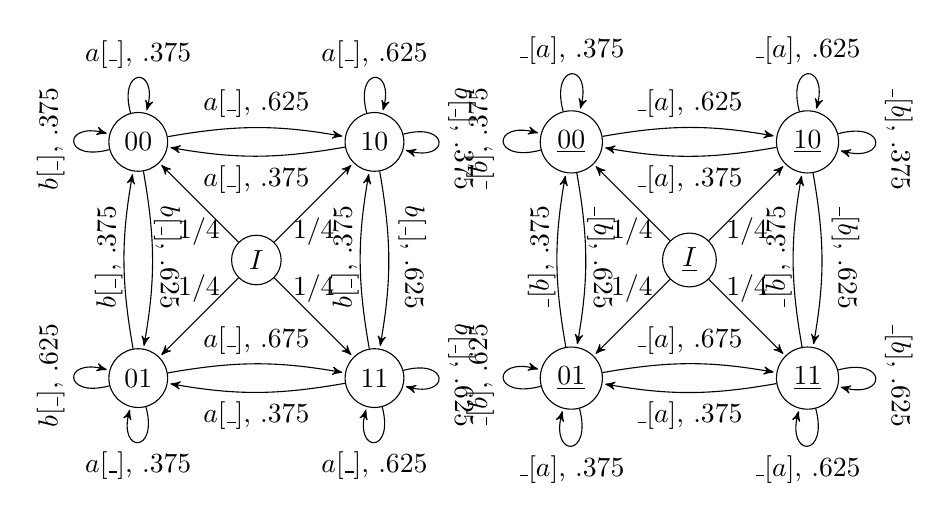
\begin{tikzpicture}[->,>=stealth',shorten >=1pt,auto,node
      distance=2cm,node/.style={circle,draw}]
      \node[node] (I) at  ( 0,  0) { $I$ };
      \node[node] (00) at (-1.5,  1.5) { $00$ };
      \node[node] (01) at (-1.5, -1.5) { $01$ };
      \node[node] (10) at ( 1.5,  1.5) { $10$ };
      \node[node] (11) at ( 1.5, -1.5) { $11$ };

      \path
      (I) edge node [below=2] { $1/4$ } (00)
      (I) edge node [above=2] { $1/4$ } (01)
      (I) edge node [below=2] { $1/4$ } (10)
      (I) edge node [above=2] { $1/4$ } (11)

      (00) edge [loop above] node { $a[\uscore]$, .375 } (00)
      (00) edge [bend left=10] node { $a[\uscore]$, .625 } (10)
      (00) edge [loop left] node [above=1,rotate=90] { $b[\uscore]$, .375 } (00)
      (00) edge [bend left=10] node [left=3,above=1,rotate=270] { $b[\uscore]$, .625 } (01)

      (10) edge [loop above] node { $a[\uscore]$, .625 } (00)
      (10) edge [bend left=10] node { $a[\uscore]$, .375 } (00)
      (10) edge [loop right] node [above=1,rotate=270] { $b[\uscore]$, .375 } (10)
      (10) edge [bend left=10] node [above=1,rotate=270] { $b[\uscore]$, .625 } (11)
     
      (11) edge [loop below] node { $a[\uscore]$, .625 } (11)
      (11) edge [bend left=10] node { $a[\uscore]$, .375 } (01)
      (11) edge [loop right] node [above=1,rotate=270] { $b[\uscore]$, .625 } (11)
      (11) edge [bend left=10] node [left=-3,above=1,rotate=90] { $b[\uscore]$, .375 } (10)
     
      (01) edge [loop below] node { $a[\uscore]$, .375 } (01)
      (01) edge [bend left=10] node { $a[\uscore]$, .675 } (11)
      (01) edge [loop left] node [above=1,rotate=90] { $b[\uscore]$, .625 } (01)
      (01) edge [bend left=10] node [left=-3,above=1,rotate=90] { $b[\uscore]$, .375 } (00)
     
      ;



      \node[node] (I') at  ( 5.5,    0) { $\underline{I}$ };
      \node[node] (00') at (   4,  1.5) { $\underline{00}$ };
      \node[node] (01') at (   4, -1.5) { $\underline{01}$ };
      \node[node] (10') at (   7,  1.5) { $\underline{10}$ };
      \node[node] (11') at (   7, -1.5) { $\underline{11}$ };

      \path
      (I') edge node [below=2] { $1/4$ } (00')
      (I') edge node [above=2] { $1/4$ } (01')
      (I') edge node [below=2] { $1/4$ } (10')
      (I') edge node [above=2] { $1/4$ } (11')

      (00') edge [loop above] node { $\uscore[a]$, .375 } (00')
      (00') edge [bend left=10] node { $\uscore[a]$, .625 } (10')
      (00') edge [loop left] node [above=1,rotate=90] { $\uscore[b]$, .375 } (00')
      (00') edge [bend left=10] node [left=3,above=1,rotate=270] { $\uscore[b]$, .625 } (01')

      (10') edge [loop above] node { $\uscore[a]$, .625 } (00')
      (10') edge [bend left=10] node { $\uscore[a]$, .375 } (00')
      (10') edge [loop right] node [above=1,rotate=270] { $\uscore[b]$, .375 } (10')
      (10') edge [bend left=10] node [above=1,rotate=270] { $\uscore[b]$, .625 } (11')
     
      (11') edge [loop below] node { $\uscore[a]$, .625 } (11')
      (11') edge [bend left=10] node { $\uscore[a]$, .375 } (01')
      (11') edge [loop right] node [above=1,rotate=270] { $\uscore[b]$, .625 } (11')
      (11') edge [bend left=10] node [left=-3,above=1,rotate=90] { $\uscore[b]$, .375 } (10')
     
      (01') edge [loop below] node { $\uscore[a]$, .375 } (01')
      (01') edge [bend left=10] node { $\uscore[a]$, .675 } (11')
      (01') edge [loop left] node [above=1,rotate=90] { $\uscore[b]$, .625 } (01')
      (01') edge [bend left=10] node [left=-3,above=1,rotate=90] { $\uscore[b]$, .375 } (00')
     
      ;
      \end{tikzpicture}
      \caption{Adjacent Inputs}
      \label{figure:adjacent-inputs}
    \end{subfigure}
    \begin{subfigure}{\columnwidth}
      \centering
      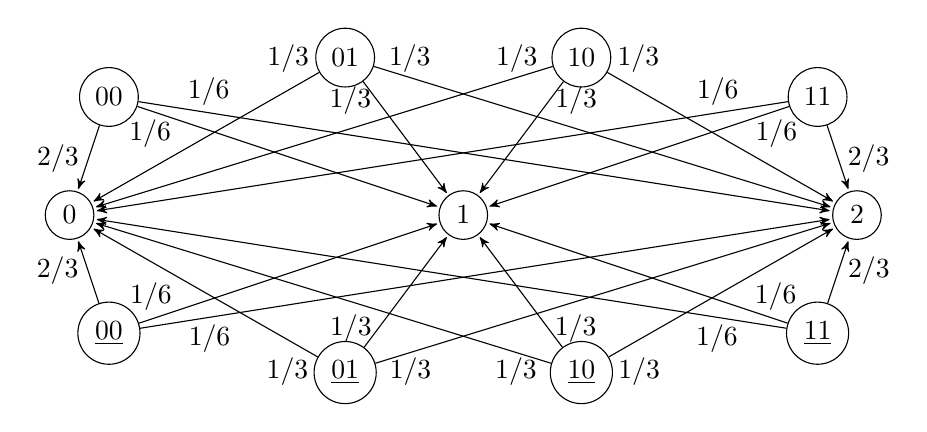
\begin{tikzpicture}[->,>=stealth',shorten >=1pt,auto,node
      distance=2cm,node/.style={circle,draw}]
      \node[node] (0) at (-5,  0) { $0$ };
      \node[node] (1) at ( 0,  0) { $1$ };
      \node[node] (2) at ( 5,  0) { $2$ };

      \node[node] (00) at (-4.5, 1.5) { $00$ };
      \node[node] (01) at (-1.5, 2) { $01$ };
      \node[node] (10) at ( 1.5, 2) { $10$ };
      \node[node] (11) at ( 4.5, 1.5) { $11$ };

      \node[node] (00') at (-4.5, -1.5) { $\underline{00}$ };
      \node[node] (01') at (-1.5, -2) { $\underline{01}$ };
      \node[node] (10') at ( 1.5, -2) { $\underline{10}$ };
      \node[node] (11') at ( 4.5, -1.5) { $\underline{11}$ };

      \path
      (00) edge node [left] { $2/3$ } (0)
      (00) edge node [left=50,above] { $1/6$ } (1)
      (00) edge node [left=100,above=15] { $1/6$ } (2)

      (01) edge node [right=30,above=20] { $1/3$ } (0)
      (01) edge node [left=20,above=5] { $1/3$ } (1)
      (01) edge node [left=70,above=20] { $1/3$ } (2)

      (10) edge node [right=70,above=20] { $1/3$ } (0)
      (10) edge node [right=20,above=5] { $1/3$ } (1)
      (10) edge node [left=30,above=20] { $1/3$ } (2)

      (11) edge node [right=100,above=15] { $1/6$ } (0)
      (11) edge node [right=50,above] { $1/6$ } (1)
      (11) edge node [right] { $2/3$ } (2)


      (00') edge node [left] { $2/3$ } (0)
      (00') edge node [left=50,below] { $1/6$ } (1)
      (00') edge node [left=100,below=15] { $1/6$ } (2)

      (01') edge node [right=30,below=20] { $1/3$ } (0)
      (01') edge node [left=20,below=5] { $1/3$ } (1)
      (01') edge node [left=70,below=20] { $1/3$ } (2)

      (10') edge node [right=70,below=20] { $1/3$ } (0)
      (10') edge node [right=20,below=5] { $1/3$ } (1)
      (10') edge node [left=30,below=20] { $1/3$ } (2)

      (11') edge node [right=100,below=15] { $1/6$ } (0)
      (11') edge node [right=50,below] { $1/6$ } (1)
      (11') edge node [right] { $2/3$ } (2)
      ;

      \end{tikzpicture}
      \caption{Randomized Frequency}
      \label{figure:randomized-frequency}
    \end{subfigure}
  \caption{Frequency Estimator}
  \label{figure:frequency-estimator}
\end{figure}

\todo{verify this is $1$-DP}

\section{Conclusions}
\label{section:conclusions}


\bibliographystyle{splncs03}
\bibliography{refs}

\end{document}
